% !TEX root = ../main.tex

\section{Mixture models}
\label{sec:mixofgauss}
The learning outcomes are as follows:
\begin{enumerate}
	\item Learn what sort of data mixture models should be used to model
	\item Perform posterior inference in a mixture model
\end{enumerate}

Mixture models are models in which we want to, I suppose, learn the \textit{label} of our particular datum. Or, in another way, we aim to associate that datum with a number of other datum which our model learns to have the same characteristics and hence find the distribution over the whole data, that characterizes this. \\

The latent variables $x$ in a mixture model correspond to a mixture component. Where the mixture component takes values in a discrete set $\{1, \ldots, K\}$. $K$ need not be fixed. 
In general, a mixture model assumes data are generated by the following process: first we sample $x$ and then we sample the observables $\y$ from a distribution that depends on the latent variables i.e $p(x,\y) = p(x)p(\y|x)$. In mixture models $p(x)$ is always a multinomial distribution. $p(\y|x)$ can take a variety of forms. In particular, it takes a Gaussian form in a 'Gaussian mixture model'. 

Mathematically we can write this as:
\begin{equation} p(\y) = \sum_{\x}p(\x)p(\y|\x) = \sum_{k=1}^{K} \pi_{k} \mathcal{N}(\y | \mu_{k},\Sigma_{k})\end{equation}
our latent parameters $\x$ in general will be a member of  $\x \in \ints / 2\ints$ and so we say $\x$ has a 1-of-$K$ representation. In which one element of the latent variables is equal to $1$ and all other elements are equal to $0$. This means that $x_{n} \in \{0,1\}$ and $\sum_{k}^{K} x_{k} = 1$.  This means that marginal distribution over $p(\x)$ is specifed in terms of the mixing coefficients $\pi_{k}$ such that $p(x_{k} = 1) = \pi_{k}$. Where $\pi_{k}$ is the $Multinomial$ distribution, which is also called the $Categorical$ distribution. Elements of the Categorical distribution must satisfy the following constraints: \begin{align}
0 \leq \{\pi_{k}\} \leq 1 \\
\sum_{K}^{k=1}\pi_{k} = 1
\end{align}
Because we use the 1-of-$K$ representation we may write the marginal distribution of the latent parameters as:
\begin{equation}
	p(\x) = \Pi_{k=1}^{K} \pi_{k}^{x_{k}}
\end{equation}

Likewise, the conditional distribution of $\y$ given a particular value of $\x$ is a Gaussian given as:
$p(\y|\x) = \Pi_{k=1}^{K}\mathcal{N}(\x | \boldmath{\mu}_{k}, \boldmath{\Sigma}_{k})^{x_{k}}$
AS $\x$ as $K-1$ zero elements, which means that the product of the terms would be $1*1*1..[\text{term where } x_{m} = 1]..*1..$. If we gave several observations points $\y_{1}, \dots, \y_{N}$ then each observations has a corresponding latent variable $\x_{1}, \ldots \x_{N}$
\subsection{Simple model}
In the first model we have the following:
\begin{align}
x \sim \textbf{Cat}(0.7,0.3) \\
y | x = 1 \sim \mathcal{N}(0,1) \\
y | x = 2 \sim \mathcal{N}(6,2)
\end{align}
therefore the marginal $p(y) = 0.7\mathcal{N}(0,1) + 0.3\cdot \mathcal{N}(6,2)$

\begin{figure}[h!]
	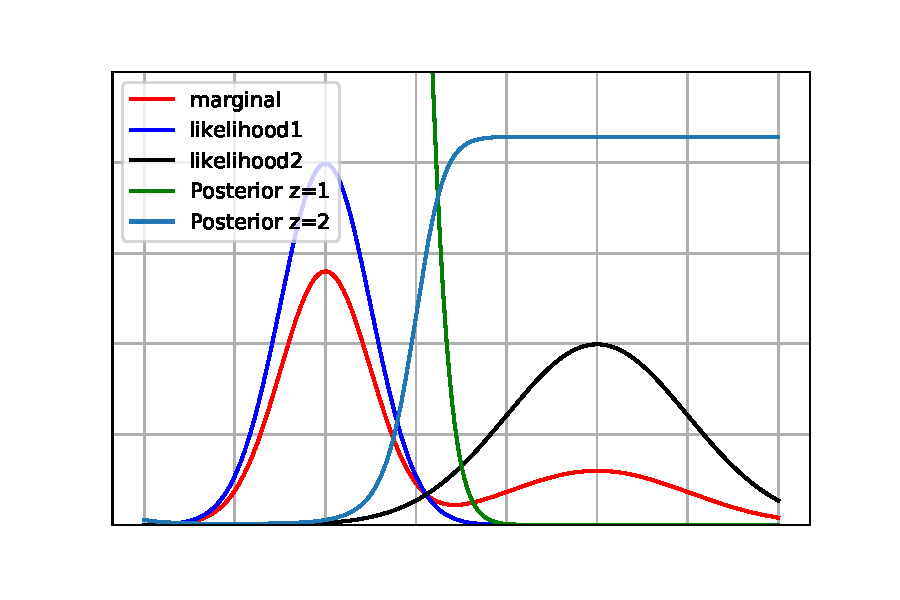
\includegraphics{code/example1.pdf}
\end{figure}

\subsection{Posterior inference}
Assuming we have already chosen the parameter models, we can infer which class a particular datum $y$ is a member of  via Bayes rule. That is $p(x|\y) \propto p(x)p(\y|x)$ and from example 1, that means that we have the following: \begin{align}
p(x=1|\y) =  \frac{p(x=1)p(\y|x=1)}{0.7\mathcal{N}(0,1) + 0.3\cdot \mathcal{N}(6,2)}
\end{align}

\subsection{Another Simple Model}
Consider the following 2-D mixture of Gaussians model, where $y_{1}$ and $y_{2}$ are conditionally independent given $x$. 
\begin{align}
x \sim \text{Cat}(0.4,0.6)\\
y_{1} | x = 1 \sim \mathcal{N}(0,1)\\
y_{2} | x = 1 \sim \mathcal{N}(6,1)\\
y_{1} | x = 2 \sim \mathcal{N}(6,2)\\
y_{2} | x = 2 \sim \mathcal{N}(3,2)
\end{align}
